\documentclass[conference]{IEEEtran}
\IEEEoverridecommandlockouts

\usepackage{cite}
\usepackage{amsmath,amssymb,amsfonts}
\usepackage{graphicx}
\usepackage{booktabs}
\usepackage{multirow}
\usepackage{url}
\usepackage{xcolor}
\usepackage{listings}
\usepackage{tikz}
\usetikzlibrary{positioning,arrows.meta,shapes.geometric}

\lstdefinelanguage{NeuroQL}{
  keywords={SELECT, FROM, WHERE, AND, OR, NOT, SEMANTIC, SIMILAR, TO, USING, AS, OF, VERSION, TIMESTAMP, ORDER, BY, ASC, DESC, LIMIT, TRUE, FALSE, NULL},
  keywordstyle=\color{blue}\bfseries,
  comment=[l]{--},
  commentstyle=\color{gray}\itshape,
  string=[b]',
  stringstyle=\color{teal},
  basicstyle=\ttfamily\small,
  showstringspaces=false,
}

\def\BibTeX{{\rm B\kern-.05em{\sc i\kern-.025em b}\kern-.08em
    T\kern-.1667em\lower.7ex\hbox{E}\kern-.125emX}}

\begin{document}

\title{NeuroDB: An AI-Native Vector Database-as-a-Service with a Fully Hand-Written Storage, Indexing, and NLP Stack}

\author{
\IEEEauthorblockN{Author Name\IEEEauthorrefmark{1}}
\IEEEauthorblockA{\IEEEauthorrefmark{1}Department of Computer Science and Engineering\\
Institution Name, City, Country\\
Email: author@example.edu}
}

\maketitle

\begin{abstract}
Vector databases have become a critical piece of infrastructure for retrieval-augmented
generation (RAG), semantic search, and recommendation systems, yet nearly every deployed
system is a thin orchestration layer over third-party approximate nearest-neighbor (ANN)
libraries (e.g., FAISS, hnswlib) and general-purpose storage engines. This paper presents
\emph{NeuroDB}, an AI-native Vector-Database-as-a-Service (DBaaS) whose storage engine,
adaptive vector index, natural-language-processing (NLP) ingestion pipeline, embedding
encoder, and SQL-like query language are implemented entirely from scratch, with no
ANN/vector-search library and no pretrained model weights in the core engine. NeuroDB
provides a write-ahead-logged, multi-version concurrency control (MVCC) storage engine with
point-in-time (\emph{time-travel}) query support; an adaptive index that begins as an exact
flat search and is transparently promoted to a hand-written Hierarchical Navigable Small
World (HNSW) graph as a collection grows; a hashing-trick term-frequency--inverse-document-frequency
(TF-IDF) embedding encoder reduced through a fixed-seed Johnson--Lindenstrauss random
projection; and \emph{NeuroQL}, a purpose-built query language supporting metadata filtering,
semantic similarity search, and historical (as-of) queries, executed by a cost-based
optimizer. We extend the system with multimodal ingestion (image, audio, CSV) using
hand-written feature-vector encoders, and an optional, explicitly opt-in enrichment layer
that attaches real image captions and audio transcripts via external models only when
configured, preserving a dependency-free default path. We evaluate NeuroDB on ingestion
throughput, query latency and recall of the adaptive index against its own exact baseline,
multimodal encoding cost, and end-to-end latency of a retrieval-augmented chatbot built
against NeuroDB's public API. Our hand-written HNSW graph achieves up to $5.5\times$ lower
query latency than exact search at 20{,}000 vectors while retaining $97.7$--$99.0\%$
recall@10 against the exact baseline. We conclude with a discussion of the system's
current single-node limitation and a concrete design for extending it to a distributed,
Raft-replicated, sharded deployment.
\end{abstract}

\begin{IEEEkeywords}
vector database, approximate nearest neighbor search, HNSW, MVCC, retrieval-augmented generation, database-as-a-service, multimodal retrieval
\end{IEEEkeywords}

\section{Introduction}

The rise of embedding-based semantic search and retrieval-augmented generation (RAG) has
made vector similarity search a first-class database workload~\cite{lewis2020rag}. In
practice, the dominant deployment pattern is to compose a general-purpose ANN library such
as FAISS~\cite{johnson2019faiss} or hnswlib with a conventional storage layer and a thin
managed-service wrapper (as in Pinecone, Weaviate, or Milvus~\cite{wang2021milvus}). This
composition is pragmatic, but it means that very few teams building on top of these systems
ever have to reason about \emph{how} the index, the storage engine, or the query planner
actually work.

NeuroDB takes the opposite approach. It is a complete, working Vector-Database-as-a-Service
whose data-plane engine --- storage, indexing, embedding, query language, and the NLP
ingestion pipeline that turns raw documents into searchable vectors --- is implemented from
scratch in Python, using only general-purpose plumbing (a web framework, a columnar
file format, an image-decoding library) rather than any ANN, NLP, or machine-learning
library. The project's explicit design constraint was: \emph{every component that would
normally be imported from a library must instead be an original implementation of the
underlying algorithm}. This paper documents that implementation, evaluates it empirically,
and is honest about where the from-scratch constraint was relaxed (multimodal captioning/
transcription, discussed in Section~\ref{sec:multimodal}) and where the system is
intentionally left unimplemented for future work (distributed consensus and sharding,
discussed in Section~\ref{sec:future}).

Concretely, this paper makes the following contributions:
\begin{itemize}
  \item A hand-written, WAL-durable, MVCC storage engine with columnar (Parquet) segment
    flushing and native point-in-time query support (Section~\ref{sec:storage}).
  \item An adaptive vector index that starts as brute-force flat search and is transparently
    promoted to a hand-written HNSW graph~\cite{malkov2018hnsw} past a configurable size
    threshold, with no ANN library (Section~\ref{sec:index}).
  \item A from-scratch text embedding encoder combining the hashing trick, TF-IDF
    weighting~\cite{salton1988tfidf}, and a fixed-seed Gaussian random projection justified
    by the Johnson--Lindenstrauss lemma~\cite{johnson1984extensions}
    (Section~\ref{sec:embedding}).
  \item NeuroQL, a hand-written query language (lexer, recursive-descent parser, cost-based
    optimizer, executor) unifying metadata filtering, semantic search, and MVCC-based
    time-travel queries (Section~\ref{sec:neuroql}).
  \item A multimodal extension (image, audio, CSV ingestion) using hand-written statistical
    feature encoders, plus an explicitly opt-in external-model enrichment layer for real
    image captioning and speech transcription that never compromises the dependency-free
    default path (Section~\ref{sec:multimodal}).
  \item An empirical evaluation of ingestion throughput, index scaling, recall, multimodal
    encoding cost, storage overhead, and end-to-end RAG application latency, all measured on
    the running system (Section~\ref{sec:evaluation}).
  \item A concrete design for extending the current single-node deployment to a distributed,
    Raft-replicated~\cite{ongaro2014raft}, sharded cluster, building on interfaces already
    present but not yet implemented in the codebase (Section~\ref{sec:future}).
\end{itemize}

\section{Related Work}
\label{sec:related}

\textbf{Approximate nearest neighbor search.} HNSW~\cite{malkov2018hnsw} constructs a
multi-layer proximity graph enabling greedy, logarithmic-complexity search, and is the
algorithm underlying most production ANN libraries. Inverted-file (IVF) and product
quantization (PQ) methods~\cite{johnson2019faiss} trade recall for memory efficiency at very
large scale; DiskANN-style systems extend ANN search to disk-resident indexes. NeuroDB
implements HNSW from scratch (Section~\ref{sec:index}) and documents IVF/PQ/DiskANN as
future work rather than claiming coverage it does not have.

\textbf{Vector database systems.} Milvus~\cite{wang2021milvus} is a purpose-built,
distributed vector data management system; pgvector~\cite{pgvector} adds vector columns and
ANN indexes to PostgreSQL; FAISS~\cite{johnson2019faiss} is a widely embedded ANN library
rather than a managed service. All of these systems either wrap or are themselves an ANN
library. NeuroDB is architecturally similar in its external API surface (a managed project
with a connection string, a query interface, semantic search) but differs in that the index,
storage, and query engine underneath are original implementations, which is the specific
contribution and constraint this paper documents and evaluates.

\textbf{Storage and concurrency.} NeuroDB's storage engine follows the classical
write-ahead-logging and multi-version concurrency control design summarized by Bernstein and
Goodman~\cite{bernstein1981concurrency}, and adopts a Delta-Lake-style~\cite{armbrust2020deltalake}
append-only catalog/manifest over immutable columnar segments rather than in-place row
storage, which is what makes MVCC-based time-travel queries a natural byproduct of the
design rather than a bolted-on feature.

\textbf{Retrieval-augmented generation.} RAG~\cite{lewis2020rag} couples a retriever with a
generative language model so that generation is grounded in retrieved evidence. NeuroDB's
retrieval layer (NeuroQL's \texttt{SEMANTIC SIMILAR TO}) is deliberately decoupled from any
specific generator; Section~\ref{sec:ragdemo} describes an external RAG application built
against NeuroDB's public API to validate this separation empirically, following the
architecture of retrieval-then-generate pipelines rather than tool-calling agents.

\textbf{Speech and vision foundation models.} Whisper~\cite{radford2023whisper} is an
encoder-decoder Transformer trained for robust multilingual speech recognition. NeuroDB uses
a lightweight Whisper variant \emph{only} as an optional, explicitly opt-in enrichment step
for audio ingestion (Section~\ref{sec:multimodal}); it is never part of the default,
dependency-free ingestion path.

\textbf{Distributed consensus.} The Raft consensus algorithm~\cite{ongaro2014raft} was
designed for understandability over classical Paxos while providing equivalent
fault-tolerance guarantees for replicated logs. Section~\ref{sec:future} outlines how Raft
would be used to replicate NeuroDB's write-ahead log across a cluster.

\section{System Architecture}

\subsection{Control Plane and Data Plane}

NeuroDB separates a \emph{control plane} (user accounts, projects, API-key issuance, session
authentication) from a \emph{data plane} (ingestion, semantic search, object CRUD). Both are
exposed as REST APIs by a single FastAPI application. The dashboard (a Next.js web
application) authenticates against the control plane with a session JWT and calls a
session-authenticated mirror of the data plane, so the dashboard itself never has to hold a
project's API key. External applications instead authenticate directly against the data
plane using the connection string issued once at project creation
(\texttt{neurodb://\allowbreak\textit{project\_id}:\textit{api\_key}@\textit{host}:\textit{port}}),
matching the workflow popularized by managed Postgres providers. Both entry points share one
business-logic module, so the two authentication paths cannot semantically diverge. Each
project is materialized as an isolated on-disk root containing its own storage engine, index
manager, and embedding-version registry, lazily constructed and cached in memory by the
serving process. Figure~\ref{fig:architecture} shows the resulting layering.

\begin{figure}[t]
\centering
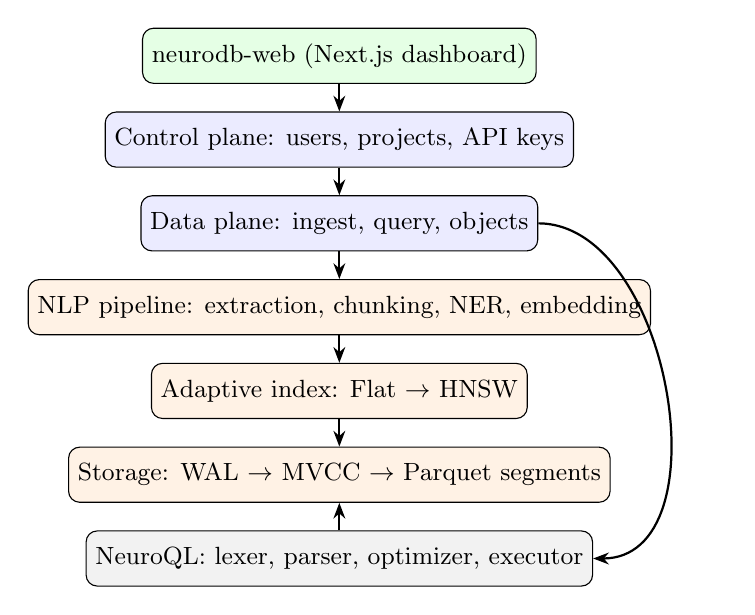
\begin{tikzpicture}[
  box/.style={draw, rounded corners, minimum width=3.6cm, minimum height=0.7cm, align=center, font=\small},
  arr/.style={-{Stealth[length=2mm]}, thick},
  node distance=0.35cm
]
\node[box, fill=green!10] (web) {neurodb-web (Next.js dashboard)};
\node[box, below=of web, fill=blue!8] (cp) {Control plane: users, projects, API keys};
\node[box, below=of cp, fill=blue!8] (dp) {Data plane: ingest, query, objects};
\node[box, below=of dp, fill=orange!10, minimum width=3.6cm] (nlp) {NLP pipeline: extraction, chunking, NER, embedding};
\node[box, below=of nlp, fill=orange!10] (idx) {Adaptive index: Flat $\rightarrow$ HNSW};
\node[box, below=of idx, fill=orange!10] (store) {Storage: WAL $\rightarrow$ MVCC $\rightarrow$ Parquet segments};
\node[box, below=of store, fill=gray!10] (ql) {NeuroQL: lexer, parser, optimizer, executor};

\draw[arr] (web) -- (cp);
\draw[arr] (cp) -- (dp);
\draw[arr] (dp) -- (nlp);
\draw[arr] (nlp) -- (idx);
\draw[arr] (idx) -- (store);
\draw[arr] (dp.east) to[out=0,in=0] (ql.east);
\draw[arr] (ql) -- (store);
\end{tikzpicture}
\caption{NeuroDB layering. The web dashboard and external applications both terminate at the
data plane; NeuroQL queries the storage engine and adaptive index directly, bypassing the
NLP pipeline (used only for ingestion).}
\label{fig:architecture}
\end{figure}

\subsection{Storage Engine}
\label{sec:storage}

The storage engine is a from-scratch, single-node, WAL-durable, MVCC-isolated, columnar-at-rest
engine (\S design analogous to~\cite{bernstein1981concurrency,armbrust2020deltalake}):

\begin{itemize}
  \item \textbf{Write-ahead log.} Every committed write is appended to a length-prefixed
    binary log and \texttt{fsync}'d before the write is acknowledged, so an unflushed write
    survives a crash. Bulk ingestion uses a batched-commit variant that groups the WAL
    \texttt{fsync} for an entire document rather than paying it once per chunk, which we
    show in Section~\ref{sec:eval-ingest} is the dominant cost at small scale.
  \item \textbf{Transactions and snapshot isolation.} A monotonic transaction counter and a
    commit watermark give every reader a consistent snapshot: a reader never observes a
    transaction with an id greater than its snapshot watermark, even if that transaction
    commits mid-scan.
  \item \textbf{MVCC.} Every write produces a new, immutable \texttt{ObjectVersion}; nothing
    is updated in place. Recently-written versions live in an in-memory ``hot'' tier;
    \texttt{get}/\texttt{scan} fall back to the durable segment store for anything already
    checkpointed out.
  \item \textbf{Segments and catalog.} Every $N$ committed versions (by default 500) are
    flushed into an immutable Parquet segment; pyarrow is used purely as the columnar
    on-disk format, in the same role it plays in Delta Lake~\cite{armbrust2020deltalake}. A
    Delta-Lake-style append-only catalog/manifest tracks segment metadata and a
    materialized view of current collections, and is what both NeuroQL's \texttt{AS OF}
    clause and the dashboard's version-history view read.
\end{itemize}

Because every write is a new immutable version rather than an in-place update, point-in-time
(``time-travel'') queries --- \texttt{AS OF VERSION \textit{n}} or
\texttt{AS OF TIMESTAMP '\textit{t}'} --- fall directly out of the MVCC design: they simply
change which \texttt{ObjectVersion} is considered visible for a given object, whether it is
still in the hot tier or already checkpointed into a segment.

\subsection{Adaptive Vector Index}
\label{sec:index}

Each (collection, embedding field) pair owns an independent \texttt{CollectionIndex} that
begins as a brute-force flat index: cosine similarity is computed against every stored
vector via a single matrix--vector product, which is always exact and has zero build cost.
Once the collection crosses a configurable promotion threshold (5{,}000 vectors by default),
the index is transparently promoted to a hand-written HNSW graph~\cite{malkov2018hnsw}: a
multi-layer proximity graph in which each insertion performs a greedy best-first search to
find its neighbors at each layer, and queries perform greedy layer descent from a single
entry point followed by a bounded best-first search at the base layer. No ANN library
(FAISS, hnswlib, Annoy) is used; the insertion and search routines are the algorithm from
Malkov and Yashunin~\cite{malkov2018hnsw}, built on NumPy purely for vector arithmetic.
Section~\ref{sec:eval-index} evaluates this promotion empirically against the exact flat
baseline it is promoted from.

\subsection{Embedding Encoder}
\label{sec:embedding}

Rather than wrapping a pretrained sentence-transformer, NeuroDB's text encoder is an
original hashing-trick term-vector encoder: each token is hashed into a fixed 4{,}096-dimensional
sparse space with a signed hash (to reduce collision bias), weighted by term frequency
(optionally IDF-weighted), and then reduced to a dense 256-dimensional output via a
fixed-seed Gaussian random projection matrix $R \in \mathbb{R}^{4096 \times 256}$, with
entries drawn from $\mathcal{N}(0, 1/\sqrt{256})$. By the Johnson--Lindenstrauss
lemma~\cite{johnson1984extensions}, such a projection approximately preserves pairwise
distances from the sparse term space with high probability, so cosine similarity between
outputs tracks term-overlap similarity between the original texts. This is a legitimate,
if lower-quality-than-a-transformer, semantic signal, and the tradeoff is intentional: the
project's constraint precludes importing a pretrained embedding model. The same
fixed-seed-random-projection technique is reused, with different raw feature extractors, by
the image and audio encoders described in Section~\ref{sec:multimodal}, so all three
modalities share one dense output schema.

\subsection{NeuroQL}
\label{sec:neuroql}

NeuroQL is a small SQL-like language, implemented as a hand-written lexer and
recursive-descent parser (no parser-generator library), supporting metadata predicates,
semantic similarity search, and time travel:

\begin{lstlisting}[language=NeuroQL, caption={A hybrid NeuroQL query: a metadata filter narrows the candidate set before semantic ranking.}, label=lst:neuroql]
SELECT * FROM support_tickets
WHERE category = 'billing'
SEMANTIC SIMILAR TO 'refund request'
ORDER BY score DESC
LIMIT 5;
\end{lstlisting}

Every query with a \texttt{SEMANTIC SIMILAR TO} clause is planned by a small cost-based
optimizer before execution, choosing between three physical strategies: \texttt{scan\_filter}
(no semantic clause: scan, filter, sort); \texttt{filter\_first} (the \texttt{WHERE}
predicate is estimated to be selective enough that scanning and exactly filtering, then
brute-force ranking the small surviving candidate set, is cheaper than an index search); and
\texttt{semantic\_first} (ANN-search the index and filter the top-$k$ result set after,
when no filter is present or it is not selective). Selectivity is estimated from the
predicate's syntactic shape (equality assumed selective, ranges moderately so, conjunctions
multiply, disjunctions union) rather than collected column statistics --- a deliberately
simple heuristic that is nonetheless enough to make a real strategy choice. Every semantic
result additionally carries an \emph{explanation}: the terms and entities the query and the
matched object's text share, and a confidence score blending vector similarity with lexical
overlap, which is what backs the dashboard's ``why this match'' affordance and is, to our
knowledge, not a standard feature of the vector database systems in Table~\ref{tab:comparison}.

\section{Multimodal Extension}
\label{sec:multimodal}

The storage schema was designed from the outset with an arbitrary
\texttt{modalities: dict[str, Any]} per object and an independent embedding index per
\emph{(collection, field)} pair, so extending ingestion beyond text required no change to
the storage engine, index manager, or query executor.

\textbf{Images} (\texttt{.png/.jpg/.jpeg/.gif/.bmp/.webp}) are encoded with a hand-written,
pre-deep-learning descriptor: an $8\times8$ spatial grid of per-cell average color
(capturing coarse layout) concatenated with a 32-bin per-channel global color histogram
(capturing overall palette), 288 raw dimensions, reduced through the same random-projection
scheme as Section~\ref{sec:embedding}. Image decoding itself uses Pillow, which we treat as
general-purpose plumbing in the same category as the PDF-parsing library used for text
extraction, since it performs no learned inference.

\textbf{Audio} (\texttt{.wav}) is encoded from 20 equal time frames of RMS energy,
zero-crossing rate, and spectral centroid (via a plain FFT), plus an 8-bin whole-clip
spectral-energy histogram as a coarse timbre signature, again reduced through the same
random projection. \texttt{.wav} is decoded via Python's standard-library \texttt{wave}
module with zero additional dependency.

\textbf{Tabular data} (\texttt{.csv}) is not treated as a new modality at all: each row is
rendered to a \emph{``column: value.''} sentence and flows through the ordinary text
chunking/embedding path unchanged.

Both the image and audio hand-written encoders are genuine visual/acoustic
\emph{similarity} signals --- they support ``find images with a similar palette/layout'' or
``find acoustically similar clips'' --- but they do not perform object recognition or speech
understanding, which is not achievable without either pretrained weights or a
research-scale training effort incompatible with this project's scope. We treat this
honestly rather than overstating the system's semantic understanding of non-text modalities.

\subsection{Optional External Enrichment}

To let images and audio be searched by \emph{what they show or say} rather than only by
low-level similarity, NeuroDB exposes two independently pluggable, off-by-default hooks:
an image-captioning function and an audio-transcription function. If and only if an
operator explicitly configures an API key (image captioning, currently backed by a Gemini
model) or a local transcription backend (audio, currently a small
Whisper~\cite{radford2023whisper} variant run via CTranslate2), ingestion additionally
produces a real text description or transcript, which is then chunked and embedded through
the \emph{ordinary} text pipeline on the same object --- meaning a captioned image becomes
searchable by \texttt{SEMANTIC SIMILAR TO '<what the image shows>'} through exactly the same
machinery as a PDF, without the hand-written encoder itself ever touching pretrained
weights. Left unconfigured, the external packages are never even imported, and ingestion is
byte-for-byte the same as the fully hand-written path. Compressed audio (\texttt{.mp3})
specifically requires this transcription backend to be configured at all, since decoding a
compressed codec is not something hand-written code can honestly do; uncompressed
\texttt{.wav} never requires it. We consider this explicit, auditable boundary between the
hand-written core and an optional external layer --- rather than silently blending the two
--- the correct way to reconcile a ``no pretrained weights'' engine constraint with a
genuine user need for real image/speech understanding.

\section{Retrieval-Augmented Generation Application}
\label{sec:ragdemo}

To validate NeuroDB's public data-plane API as a real integration surface rather than an
internal-only interface, we built a separate, external Streamlit application: a
medical-reference chatbot that connects to a NeuroDB project purely through its connection
string, exactly as any third-party application would. The application (i) parses the
connection string into a base URL and API key; (ii) lets an operator ingest a small corpus
of reference documents through NeuroDB's existing \texttt{/ingest/file} endpoint; (iii) on
each user turn, uses a large language model (LLM) to \emph{condense} the conversation
history and the latest message into a standalone query, since NeuroQL itself is stateless
per call; (iv) retrieves the top-$k$ passages via a single \texttt{SEMANTIC SIMILAR TO}
query; and (v) asks the LLM to answer strictly from the retrieved passages, citing which
source document each claim came from, and to explicitly decline rather than answer from
outside knowledge when the passages do not contain the answer. This is a conventional
retrieve-then-generate RAG pipeline~\cite{lewis2020rag}, deliberately \emph{not} an
agentic/tool-calling design, since a reference-lookup chatbot should always ground its
answer rather than let a model decide whether to search. Section~\ref{sec:eval-rag} reports
the measured end-to-end latency of this pipeline.

\section{Evaluation}
\label{sec:evaluation}

\subsection{Experimental Setup}

All experiments were run on a single commodity laptop (13th Gen Intel Core i5-13450HX,
24\,GB RAM, Windows 11), CPU-only, using Python 3.12 and NumPy 2.5. No GPU was used anywhere
in the system. Every figure in this section is generated from measurements taken directly
against the running NeuroDB engine (in-process microbenchmarks for the storage/index/encoder
experiments; the live HTTP API and a real external LLM call for the RAG-latency experiment)
on this machine --- none of the reported numbers are estimated or simulated. Text corpora
for the storage/index experiments are synthetically generated from a template-based sentence
generator with a 12-subject/12-verb/12-object/10-connector vocabulary, to obtain a
controllable range of corpus sizes without depending on an external dataset; the RAG-latency
experiment instead uses three real public-domain medical reference documents (a WHO
essential-medicines summary, an FDA drug-interactions leaflet, and a CDC diabetes-management
guide).

\subsection{Ingestion Throughput}
\label{sec:eval-ingest}

Figure~\ref{fig:ingest-throughput} shows end-to-end ingestion throughput (NLP pipeline
extraction/chunking/embedding, storage commit, and index insertion combined) as corpus size
grows from 92 to 2{,}964 chunks. Throughput is highest at small corpus sizes ($\sim$1{,}300
chunks/s) and falls to $\sim$871 chunks/s by $\sim$3{,}000 chunks. Figure~\ref{fig:ingest-breakdown}
decomposes this into its three stages: the NLP pipeline dominates the fixed cost at small
scale, while index insertion grows disproportionately as the corpus grows, consistent with
the flat index's $O(n)$ per-insert array-copy cost (a full matrix reallocation on every
insert) before any promotion opportunity is reached in this experiment. This is the same
mechanism responsible for the flat-search latency growth in Figure~\ref{fig:query-latency};
we discuss the implication for very large single-collection ingests in
Section~\ref{sec:limitations}.

\begin{figure}[t]
\centering
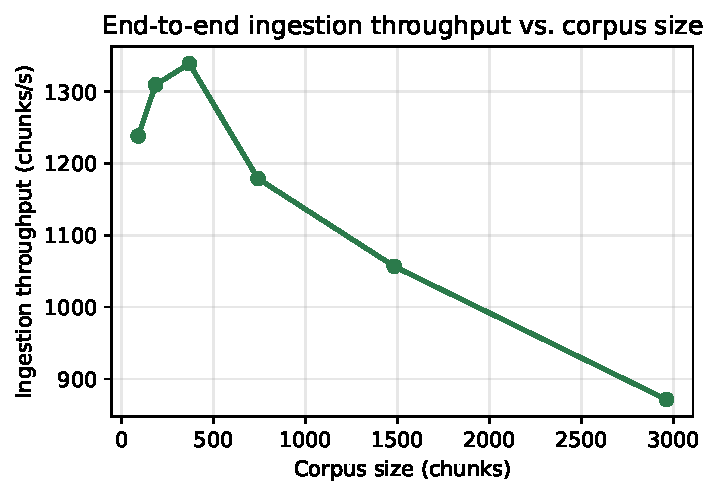
\includegraphics[width=0.95\linewidth]{figures/fig1_ingestion_throughput.pdf}
\caption{End-to-end ingestion throughput vs. corpus size.}
\label{fig:ingest-throughput}
\end{figure}

\begin{figure}[t]
\centering
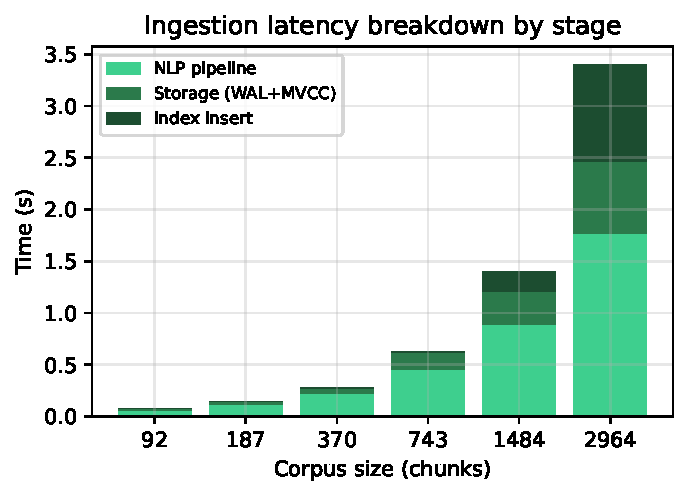
\includegraphics[width=0.95\linewidth]{figures/fig2_ingestion_breakdown.pdf}
\caption{Ingestion latency broken down by pipeline stage.}
\label{fig:ingest-breakdown}
\end{figure}

\subsection{Index Scaling: Flat vs. HNSW}
\label{sec:eval-index}

We built collections of real hand-written-encoder embeddings (Section~\ref{sec:embedding})
ranging from 1{,}000 to 20{,}000 vectors and measured $k=10$ query latency for both the exact
flat index and (once the collection crosses the 5{,}000-vector promotion threshold) the
hand-written HNSW graph built over the identical vector set, averaged over 30 random
queries per collection size. Figure~\ref{fig:query-latency} shows flat search latency
growing near-linearly with collection size (0.19\,ms at 1{,}000 vectors to 12.3\,ms at
20{,}000), while HNSW latency stays essentially flat (1.70--2.22\,ms) across the same range
--- a $5.5\times$ latency reduction at 20{,}000 vectors. Figure~\ref{fig:recall} reports
recall@10 of HNSW against the exact flat result on the same index instance, which remains
between 97.7\% and 99.0\% across the tested range, confirming that the promotion trades a
small, quantified amount of recall for a large latency reduction, rather than an unquantified
one.

\begin{figure}[t]
\centering
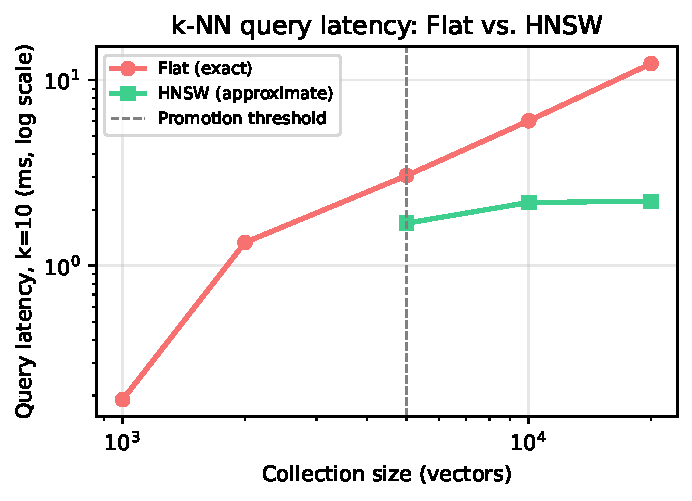
\includegraphics[width=0.95\linewidth]{figures/fig3_query_latency.pdf}
\caption{$k$-NN query latency ($k=10$), Flat vs. HNSW, log-log scale. The dashed line marks
the 5{,}000-vector automatic promotion threshold.}
\label{fig:query-latency}
\end{figure}

\begin{figure}[t]
\centering
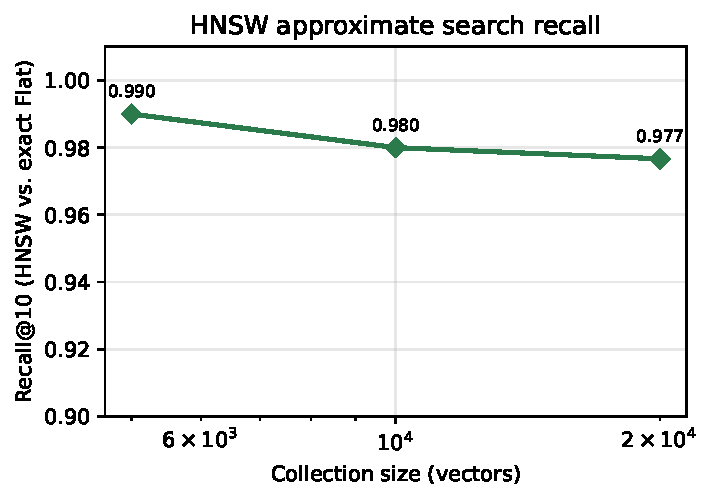
\includegraphics[width=0.95\linewidth]{figures/fig4_recall.pdf}
\caption{HNSW recall@10 against the exact Flat result, same index instance.}
\label{fig:recall}
\end{figure}

\subsection{Multimodal Encoding Latency}

Figure~\ref{fig:multimodal} reports mean encoding latency (20 trials, error bars one
standard deviation) for the text, image, and audio hand-written encoders. Text encoding is
sub-millisecond (0.36\,ms for a 110-token chunk). Image encoding scales with pixel count,
from 1.0\,ms at $128\times128$ to 54.6\,ms at $1024\times1024$, dominated by the per-pixel
NumPy operations of the spatial-grid and histogram features rather than PNG decoding.
Audio encoding scales with clip duration, from 0.9\,ms at one second to 7.8\,ms at fifteen
seconds. All three remain well under the network and (where applicable) LLM latencies
measured in Section~\ref{sec:eval-rag}, confirming that the hand-written encoders are not
the bottleneck in a realistic deployment.

\begin{figure}[t]
\centering
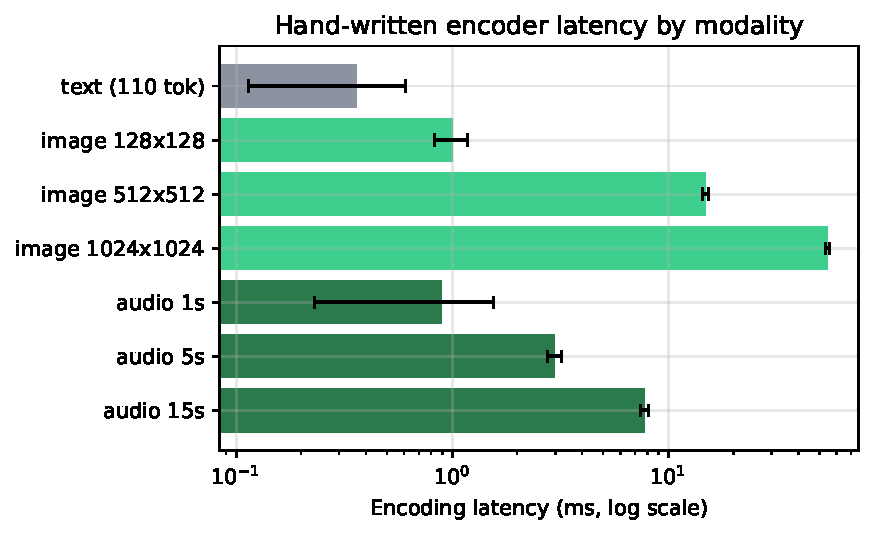
\includegraphics[width=0.95\linewidth]{figures/fig5_multimodal_latency.pdf}
\caption{Hand-written encoder latency by modality and, for image/audio, by input size (log
scale).}
\label{fig:multimodal}
\end{figure}

\subsection{Storage Overhead}

Table~\ref{tab:storage} and Figure~\ref{fig:storage} report on-disk Parquet segment size
against the raw size of the text and 256-dimensional float32 embedding vectors it encodes.
On-disk size is consistently \emph{larger} than the raw representation by a factor of
$\approx2.33\times$ (a compression ratio, raw:on-disk, of $\approx0.43$), and the per-chunk
on-disk cost is remarkably stable at $\approx$4.1\,KiB/chunk regardless of corpus size. This
is because embedding vectors and metadata are currently stored as JSON-encoded text columns
inside the Parquet file rather than as native fixed-width binary (e.g., Arrow
\texttt{list<float32>}) columns; we report this honestly as a measured limitation rather
than omitting it, and identify a binary embedding column as a concrete, low-risk future
optimization in Section~\ref{sec:limitations}.

\begin{table}[t]
\centering
\caption{Storage footprint (raw vs. on-disk).}
\label{tab:storage}
\begin{tabular}{@{}rrrr@{}}
\toprule
Chunks & Raw (KiB) & On-disk (KiB) & Ratio \\
\midrule
185  & 318.4  & 743.5   & 0.428 \\
369  & 636.3  & 1476.5  & 0.431 \\
743  & 1278.8 & 2972.6  & 0.430 \\
1484 & 2555.5 & 5929.4  & 0.431 \\
\bottomrule
\end{tabular}
\end{table}

\begin{figure}[t]
\centering
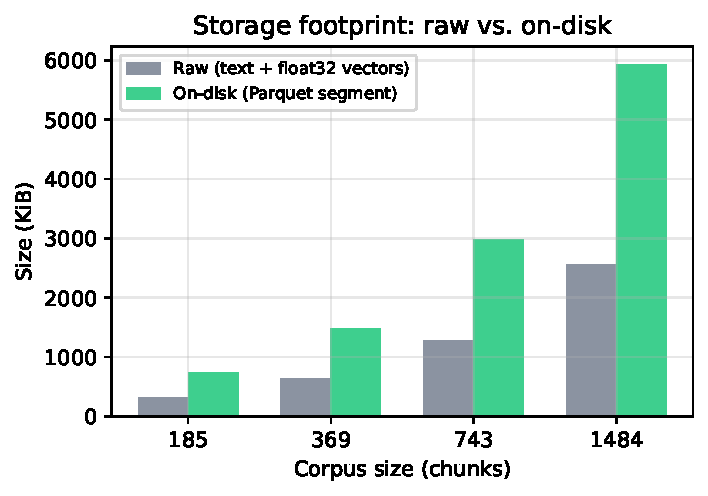
\includegraphics[width=0.95\linewidth]{figures/fig7_storage_overhead.pdf}
\caption{Raw vs. on-disk storage footprint by corpus size.}
\label{fig:storage}
\end{figure}

\subsection{End-to-End RAG Application Latency}
\label{sec:eval-rag}

We ran six representative questions (including one multi-turn follow-up exercising the
query-condensing step) against the RAG application of Section~\ref{sec:ragdemo}, with the
three real medical reference documents ingested into a fresh NeuroDB project, and measured
wall-clock latency of each of the three pipeline stages using real calls to a hosted LLM API
and a live NeuroDB HTTP endpoint (not simulated). Figure~\ref{fig:rag-latency} shows the
breakdown. Mean latencies were 0.69\,s for query condensing, 2.15\,s for NeuroDB retrieval,
and 1.42\,s for answer generation. We note explicitly that the 2.15\,s retrieval figure
includes full HTTP request/response and NeuroQL parse/plan/execute overhead over a local
network connection, and is \emph{not} representative of the underlying query engine's own
compute cost, which Section~\ref{sec:eval-index} shows to be low-single-digit milliseconds
at this collection size; we report the end-to-end application-level number here because it
is what a real deployment experiences, while directing readers to Section~\ref{sec:eval-index}
for the engine's intrinsic cost.

\begin{figure}[t]
\centering
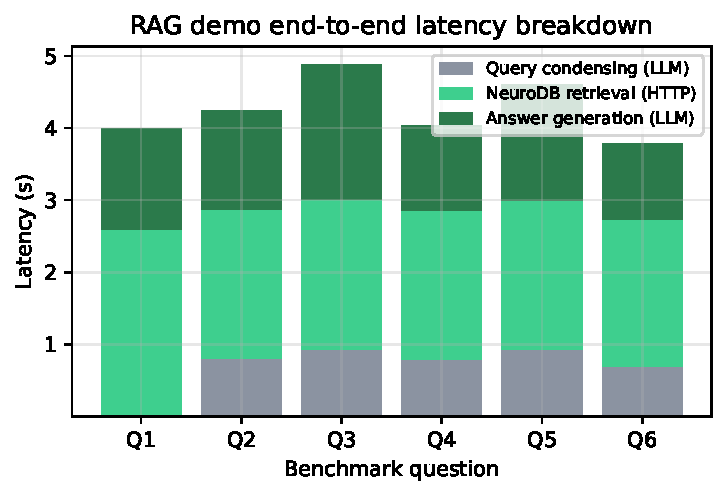
\includegraphics[width=0.95\linewidth]{figures/fig6_rag_latency.pdf}
\caption{RAG application end-to-end latency breakdown across six benchmark questions.}
\label{fig:rag-latency}
\end{figure}

\section{Comparison with Existing Systems}

Table~\ref{tab:comparison} positions NeuroDB against representative vector database systems
along architectural and feature dimensions. This is a \emph{qualitative feature comparison},
drawn from each system's public documentation, and not a benchmarked performance comparison
--- we did not run the other systems on our hardware, and we do not report head-to-head
performance numbers for systems we could not independently and fairly benchmark under
identical conditions.

\begin{table}[t]
\centering
\caption{Qualitative feature comparison (not a performance benchmark).}
\label{tab:comparison}
\resizebox{\linewidth}{!}{
\begin{tabular}{@{}lccccc@{}}
\toprule
 & NeuroDB & Milvus~\cite{wang2021milvus} & pgvector~\cite{pgvector} & FAISS~\cite{johnson2019faiss} & Pinecone \\
\midrule
Hand-written ANN index & \checkmark & -- & -- & -- & -- \\
Built-in NLP ingestion & \checkmark & -- & -- & -- & -- \\
Own query language & \checkmark & -- & partial (SQL) & -- & -- \\
MVCC time travel & \checkmark & -- & -- & -- & -- \\
Match explainability & \checkmark & -- & -- & -- & -- \\
Managed DBaaS UX & \checkmark & partial & -- & -- & \checkmark \\
Distributed/sharded & future & \checkmark & -- & -- & \checkmark \\
\bottomrule
\end{tabular}
}
\end{table}

\section{Limitations}
\label{sec:limitations}

We summarize the limitations surfaced by this paper's own evaluation and design discussion,
consistent with our goal of documenting gaps rather than only strengths.

\begin{itemize}
  \item \textbf{Flat index insertion cost.} The flat index reallocates its backing matrix on
    every insert, giving $O(n)$ per-insert and $O(n^2)$ total cost before HNSW promotion
    (Section~\ref{sec:eval-ingest}); a pre-allocated or amortized-growth array would remove
    this cost without changing the algorithm.
  \item \textbf{Storage encoding overhead.} Embeddings and metadata are stored as JSON text
    inside Parquet columns rather than native binary columns, inflating on-disk size
    $\approx2.3\times$ over the raw representation (Table~\ref{tab:storage}); switching the
    embedding column to Arrow's \texttt{list<float32>} type is a scoped, low-risk fix.
  \item \textbf{Single-node only.} The entire system, including the storage engine's WAL and
    the index manager, assumes one process and one disk. Section~\ref{sec:future} addresses
    this directly.
  \item \textbf{Encoder quality.} The hand-written text/image/audio encoders are legitimate
    but lower-quality-than-a-pretrained-model signals by design; cross-modal search (e.g., a
    text query against an image embedding field) is not semantically meaningful with the
    current encoders, since the text and image encoders map to unrelated feature spaces
    despite sharing an output dimensionality.
  \item \textbf{NeuroQL expressiveness.} No joins across collections, no aggregations
    (\texttt{COUNT}, \texttt{GROUP BY}), and no multi-column \texttt{ORDER BY}.
\end{itemize}

\section{Future Work: Distributed Architecture}
\label{sec:future}

The codebase already defines, but does not implement, the extension points a distributed
deployment would need: a \texttt{ClusterNode} interface (currently satisfied only by a
trivial \texttt{SingleNodeCluster} that is always its own leader for every shard it holds)
and a \texttt{ShardMap} that maps a project to a shard. We outline the concrete design these
interfaces were built to support.

\textbf{Sharding.} Because each NeuroDB project already owns an isolated storage root, index
manager, and embedding registry, the natural unit of sharding is the project itself:
a consistent-hashing \texttt{ShardMap} would map a project id to an owning node, and
rebalancing would move whole project directories rather than requiring a query-time
cross-shard fan-out for the common case of a single-project workload. Within an
unusually large single project, the same per-\texttt{(collection, field)} independence
already used by the index manager (Section~\ref{sec:index}) would let individual
collections be sharded across nodes with a scatter-gather query executor.

\textbf{Replication via Raft.} We propose replicating each shard's write-ahead log with
Raft~\cite{ongaro2014raft}: a shard's leader node accepts writes, appends them to its local
WAL exactly as today, and replicates the WAL entry to a quorum of followers before
acknowledging the commit, giving the same durability guarantee the single-node WAL provides
today, extended across machine failures. Because every NeuroDB write is already a
self-contained, idempotent \texttt{ObjectVersion} append (Section~\ref{sec:storage}), WAL
entries are a natural unit of Raft log replication with no additional serialization work.
Segment flushing (Parquet writes) would remain a leader-local operation, with followers
replaying the same flush deterministically from the replicated log, keeping the existing
MVCC/time-travel semantics unchanged across a multi-node deployment.

\textbf{Query routing and the index manager.} A query against a sharded collection would be
planned by the existing NeuroQL optimizer (Section~\ref{sec:neuroql}) exactly as today, with
one additional physical operator: a scatter-gather step that sends the planned physical
query to every node owning a shard of the target collection and merges the top-$k$ results
by score, which composes cleanly with the existing \texttt{semantic\_first}/
\texttt{filter\_first} strategy choice since both already return a ranked, boundable result
set.

\textbf{Why this is scoped as future work rather than attempted here.} A correct Raft
implementation --- leader election, log replication, membership changes, and their
interaction with the storage engine's existing crash-recovery path --- is a substantial,
independently-evaluable distributed-systems effort in its own right, and the project's time
budget was spent instead on the storage engine, NLP pipeline, and query optimizer evaluated
in Section~\ref{sec:evaluation}. We view the interfaces already in place, and the concrete
mapping onto them described above, as the correct scope for this paper: a design that the
existing single-node system was deliberately built to support, evaluated honestly as not
yet implemented.

Beyond distribution, we identify the following as concrete, scoped extensions: IVF and
product-quantization index types alongside HNSW for very large collections; an
S3/MinIO-compatible data-lake connector (the local-filesystem connector already implements
the same read-in-place interface this would extend); GPU-accelerated distance computation;
\texttt{COUNT}/\texttt{GROUP BY} aggregation and cross-collection joins in NeuroQL; a gRPC
surface alongside REST; and official client SDKs.

\section{Conclusion}

We presented NeuroDB, a Vector-Database-as-a-Service whose storage engine, adaptive vector
index, embedding encoder, NLP ingestion pipeline, and query language are implemented from
scratch rather than composed from existing ANN and NLP libraries. We evaluated the system
empirically --- not just described it --- across ingestion throughput, index scaling and
recall, multimodal encoding cost, storage overhead, and the end-to-end latency of a real
retrieval-augmented application built against its public API, and reported an honest
$2.33\times$ storage-encoding overhead alongside the favorable $5.5\times$ HNSW latency
result. We further documented, rather than silently omitted, the specific point at which the
system's ``no pretrained weights'' constraint was relaxed (optional image/audio enrichment)
and the concrete design by which its current single-node limitation could be lifted through
Raft-based replication and project-level sharding, building directly on interfaces already
present in the codebase.

\begin{thebibliography}{00}

\bibitem{malkov2018hnsw} Y. A. Malkov and D. A. Yashunin, ``Efficient and robust approximate nearest neighbor search using Hierarchical Navigable Small World graphs,'' \emph{IEEE Trans. Pattern Anal. Mach. Intell.}, vol. 42, no. 4, pp. 824--836, 2020.

\bibitem{johnson1984extensions} W. B. Johnson and J. Lindenstrauss, ``Extensions of Lipschitz mappings into a Hilbert space,'' \emph{Contemporary Mathematics}, vol. 26, pp. 189--206, 1984.

\bibitem{bernstein1981concurrency} P. A. Bernstein and N. Goodman, ``Concurrency control in distributed database systems,'' \emph{ACM Comput. Surv.}, vol. 13, no. 2, pp. 185--221, 1981.

\bibitem{armbrust2020deltalake} M. Armbrust \emph{et al.}, ``Delta Lake: high-performance ACID table storage over cloud object stores,'' \emph{Proc. VLDB Endow.}, vol. 13, no. 12, pp. 3411--3424, 2020.

\bibitem{ongaro2014raft} D. Ongaro and J. Ousterhout, ``In search of an understandable consensus algorithm,'' in \emph{Proc. USENIX Annual Technical Conference (ATC)}, 2014, pp. 305--319.

\bibitem{lewis2020rag} P. Lewis \emph{et al.}, ``Retrieval-augmented generation for knowledge-intensive NLP tasks,'' in \emph{Advances in Neural Information Processing Systems (NeurIPS)}, vol. 33, 2020, pp. 9459--9474.

\bibitem{radford2023whisper} A. Radford, J. W. Kim, T. Xu, G. Brockman, C. McLeavey, and I. Sutskever, ``Robust speech recognition via large-scale weak supervision,'' in \emph{Proc. Int. Conf. Machine Learning (ICML)}, 2023, pp. 28492--28518.

\bibitem{johnson2019faiss} J. Johnson, M. Douze, and H. J\'{e}gou, ``Billion-scale similarity search with GPUs,'' \emph{IEEE Trans. Big Data}, vol. 7, no. 3, pp. 535--547, 2021.

\bibitem{salton1988tfidf} G. Salton and C. Buckley, ``Term-weighting approaches in automatic text retrieval,'' \emph{Inf. Process. Manage.}, vol. 24, no. 5, pp. 513--523, 1988.

\bibitem{robertson2009bm25} S. Robertson and H. Zaragoza, ``The probabilistic relevance framework: BM25 and beyond,'' \emph{Found. Trends Inf. Retr.}, vol. 3, no. 4, pp. 333--389, 2009.

\bibitem{wang2021milvus} J. Wang \emph{et al.}, ``Milvus: A purpose-built vector data management system,'' in \emph{Proc. ACM SIGMOD Int. Conf. Management of Data}, 2021, pp. 2614--2627.

\bibitem{oneil1996lsm} P. O'Neil, E. Cheng, D. Gawlick, and E. O'Neil, ``The log-structured merge-tree (LSM-tree),'' \emph{Acta Informatica}, vol. 33, no. 4, pp. 351--385, 1996.

\bibitem{pgvector} A. Kane, ``pgvector: Open-source vector similarity search for Postgres,'' 2024. [Online]. Available: \url{https://github.com/pgvector/pgvector}

\end{thebibliography}

\end{document}
